\newpage{\clearpage}
\chapter{Resultados del proyecto}

\section{Primer Prueba}

Se procedió a realizar la primer prueba con nuestro medidor y debido que en ese momento el mundo se encontrabá en la pandemia del COVID-19, tocó realizar pruebas con cargas domésticas las culaes fueron las siguientes:
\begin{itemize}
    \itemsep0em
    \item Bombillo de 9 W.
    \item Portatil dell.
    \item Osciloscopio.
    \item Raspberry.
    \item TV de 111 W.
    \item Play Station 3,
    \item Parlantes.
    \item Licuadora.
    \item Licuadora Nutribullet.
    \item Plancha de 1000 W.
\end{itemize}

% % \begin{table} [H]
% %     \begin{center}
% %         \begin{tabular}{ |c|c|c| }
% %             \hline
% %             \multirow{2}{1cm}{CARGA} & MULTÍMETRO & \multicolumn{2}{ c| }{TARJETA}\\ \cline{2-3} 
% %             & Corriente  & Voltaje\\
% %             \hline
% %             % \multicolumn{2}{ c| }{Multimetro} \\ 
% %             % \cline{2-3}
% %             Bombillo led de 9 W & 0,0772 \\
% %             % \hline 
% %             % Corriente (A) & 0.552 & 0.558 \\
% %             % \hline
% %             % Voltaje (V) & 0.00105 & 0.00105\\
% %             \hline
% %         \end{tabular}
% %     \end{center}
% %     \caption{Corriente vs Voltaje en la resistencia shunt A}
% %     \label{tab:shuntA}
% % \end{table}
\begin{table}[htbp]
    \centering
    \caption{Add caption}
      \begin{tabular}{|l|r|r|r|}
      \toprule
      \multicolumn{1}{|c|}{\multirow{2}[4]{*}{CARGA}} & \multicolumn{1}{c|}{MULTÍMETRO} & \multicolumn{2}{c|}{TARJETA} \\
  \cmidrule{2-4}          & \multicolumn{1}{l|}{Corriente} & \multicolumn{1}{l|}{Voltaje} & \multicolumn{1}{l|}{Corriente} \\
      \midrule
      Bombillo led de 9WT & 0,0772 & 122   & 0,84175682 \\
      \midrule
      Portatil, osciloscopio, Raspberry, TV(111W), Play 3, Parlantes & 1,4   & 122   & 2,48453856 \\
      \midrule
      Licuadora & 2,11  & 122   & 3,10783076 \\
      \midrule
      Licuadora pequeña & 1,46  & 122   & 2,32913756 \\
      \midrule
      Licuadora + licuadora pequeña & 3,87  & 121   & 5,06727028 \\
      \midrule
      Plancha de 1000W & 9,2   & 118   & 10,7248316 \\
      \midrule
      Licuadora + licuadora pequeña + plancha & 12,55 & 116   & 14,6785336 \\
      \bottomrule
      \end{tabular}%
    \label{tab:addlabel}%
  \end{table}%
  

  \begin{table}[htbp]
    \centering
      \begin{tabular}{|c|c|r|r|r|r|}
      \toprule
      \multicolumn{2}{|c|}{OSCILOSCOPIO} & \multicolumn{2}{c|}{\cellcolor[rgb]{ .557,  .663,  .859}Diferencias de corriente (A)} & \multicolumn{2}{c|}{\cellcolor[rgb]{ .557,  .663,  .859}Diferencia de voltaje(V)} \\
      \midrule
      \multicolumn{2}{|c|}{Voltaje} & \multicolumn{1}{c|}{\cellcolor[rgb]{ .557,  .663,  .859}Error Absoluto} & \multicolumn{1}{c|}{\cellcolor[rgb]{ .557,  .663,  .859}Error relativo} & \multicolumn{1}{c|}{\cellcolor[rgb]{ .557,  .663,  .859}Error Absoluto} & \multicolumn{1}{c|}{\cellcolor[rgb]{ .557,  .663,  .859}Error relativo} \\
      \midrule
      \multicolumn{2}{|c|}{119,93} & \cellcolor[rgb]{ .557,  .663,  .859}0,764556821 & \cellcolor[rgb]{ .557,  .663,  .859}990\% & \cellcolor[rgb]{ .557,  .663,  .859}2,07 & \cellcolor[rgb]{ .557,  .663,  .859}2\% \\
      \midrule
      \multicolumn{2}{|c|}{119,53} & \cellcolor[rgb]{ .557,  .663,  .859}1,084538555 & \cellcolor[rgb]{ .557,  .663,  .859}77\% & \cellcolor[rgb]{ .557,  .663,  .859}2,47 & \cellcolor[rgb]{ .557,  .663,  .859}2\% \\
      \midrule
      \multicolumn{2}{|c|}{119,63} & \cellcolor[rgb]{ .557,  .663,  .859}0,997830763 & \cellcolor[rgb]{ .557,  .663,  .859}47\% & \cellcolor[rgb]{ .557,  .663,  .859}2,37 & \cellcolor[rgb]{ .557,  .663,  .859}2\% \\
      \midrule
      \multicolumn{2}{|c|}{119,87} & \cellcolor[rgb]{ .557,  .663,  .859}0,869137564 & \cellcolor[rgb]{ .557,  .663,  .859}60\% & \cellcolor[rgb]{ .557,  .663,  .859}2,13 & \cellcolor[rgb]{ .557,  .663,  .859}2\% \\
      \midrule
      \multicolumn{2}{|c|}{118,56} & \cellcolor[rgb]{ .557,  .663,  .859}1,197270279 & \cellcolor[rgb]{ .557,  .663,  .859}31\% & \cellcolor[rgb]{ .557,  .663,  .859}2,44 & \cellcolor[rgb]{ .557,  .663,  .859}2\% \\
      \midrule
      \multicolumn{2}{|c|}{120} & \cellcolor[rgb]{ .557,  .663,  .859}1,524831581 & \cellcolor[rgb]{ .557,  .663,  .859}17\% & \cellcolor[rgb]{ .557,  .663,  .859}-2 & \cellcolor[rgb]{ .557,  .663,  .859}2\% \\
      \midrule
      \multicolumn{2}{|c|}{114,5} & \cellcolor[rgb]{ .557,  .663,  .859}2,128533554 & \cellcolor[rgb]{ .557,  .663,  .859}17\% & \cellcolor[rgb]{ .557,  .663,  .859}1,5 & \cellcolor[rgb]{ .557,  .663,  .859}1\% \\
      \midrule
      \multicolumn{2}{|c|}{**Promedio de diferencia =} & \cellcolor[rgb]{ .557,  .663,  .859}1,22381416 & \cellcolor[rgb]{ .557,  .663,  .859}177\% & \cellcolor[rgb]{ .557,  .663,  .859}1,568571429 & \cellcolor[rgb]{ .557,  .663,  .859}2\% \\
      \bottomrule
      \end{tabular}%
    \label{tab:addlabel}%
  \end{table}%

  **El valor de referencia es el osciloscopio o muiltimetro y el experimental es el valor de la tarjeta\\

  \begin{figure}[H]
    \begin{center}
        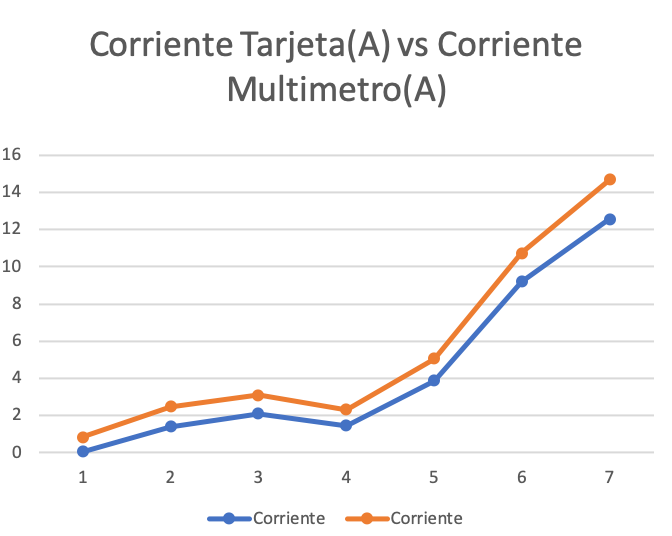
\includegraphics[width = 10cm]{4Resultados/prueba-1.png}
        \caption{ Corriente Tarjeta vs Corriente Multímetro } 
        \label{fig:prueba1}
   \end{center}
\end{figure}
  
  